No firm reports GPUs separately, so the restatement estimates a GPU asset base. Each year's cash
capital expenditure from XBRL is multiplied by the share that is servers and network equipment
(0.6 in the baseline, 0.4 and 0.8 as alternatives; no firm discloses it) and by the GPU share of
server spending (0.3 to 0.8). For Microsoft in fiscal \nAcctMsftFy, for example, \$\nAcctMsftCapexBn{}
billion of capital expenditure becomes a GPU base of \$\nAcctMsftGpuCapexBn{} billion at a GPU share
of one half. Each year's purchases form a cohort from fiscal 2020, depreciated under the firm's
disclosed straight-line life (Table~\ref{tab:lives}; changes applied prospectively, as the firms
did) and under each alternative schedule. The change in operating income is the negative of the
change in depreciation; the change in diluted EPS applies the firm-year effective tax rate.
Every firm-year number traces to an XBRL fact listed with its accession number in the replication
package.

Table~\ref{tab:restate} reports the latest fiscal year for each firm. Under the rental-implied
schedule built on the realized cohort paths, which depreciates slower than any of the disclosed
lives, the five hyperscalers' operating income would be \nAcctRealOiPctLo--\nAcctRealOiPctHi{}
\emph{higher} (\$\nAcctRealOiBnLo--\nAcctRealOiBnHi{} billion) at a GPU share of one half. Under
the steepest schedule, strategy 4 with an assumed decline of 0.40 log points a year, the change
ranges from \nAcctFourFortyOiPctLo{} to \nAcctFourFortyOiPctHi{}; the largest cut is
\nAcctFourFortyWorstFirm's, \nAcctFourFortyWorstPct{} of fiscal \nAcctFourFortyWorstFy{} operating
income, or \$\nAcctFourFortyWorstEps{} per diluted share. A four-year straight-line life gives a
similar range (\nAcctSlFourOiPctLo{} to \nAcctSlFourOiPctHi). CoreWeave and Nebius, whose operating
income is small relative to their GPU spending, are shown in dollars only.

\begin{table}[htbp]
\centering
\caption{Change in operating income and diluted EPS under alternative GPU depreciation schedules,
latest fiscal year}
\label{tab:restate}
\begin{adjustbox}{max width=\textwidth}
% Generated by src/gel/accounting/restate.py from paper/tables/p7_restatement.csv; do not edit.
\begin{tabular}{llrrrrrrrrr}
\hline
Firm & FY & SL 3y & SL 4y & SL 5y & SL 5.5y & SL 6y & M1 & M2 & M3 & M4 \\
\hline
\multicolumn{11}{l}{\textit{Panel A: change in operating income, USD bn}} \\
MSFT & 2026 & $-$4.80 to $-$12.79 & $-$2.69 to $-$7.17 & $-$1.27 to $-$3.39 & $-$0.70 to $-$1.87 & $-$0.23 to $-$0.60 & +2.56 to +6.83 & +3.45 to +9.20 & +0.30 to +0.81 & $-$2.55 to $-$6.80 \\
GOOGL & 2025 & $-$3.59 to $-$9.56 & $-$2.36 to $-$6.29 & $-$1.38 to $-$3.67 & $-$0.98 to $-$2.61 & $-$0.65 to $-$1.73 & +2.02 to +5.39 & +2.76 to +7.36 & +0.19 to +0.51 & $-$2.07 to $-$5.52 \\
AMZN & 2025 & $-$0.24 to $-$0.65 & +0.91 to +2.42 & +1.69 to +4.50 & +2.32 to +6.18 & +2.84 to +7.57 & +7.44 to +19.84 & +8.51 to +22.70 & +4.74 to +12.63 & +1.59 to +4.23 \\
META & 2025 & $-$2.46 to $-$6.56 & $-$1.86 to $-$4.96 & $-$1.04 to $-$2.77 & $-$0.68 to $-$1.82 & $-$0.39 to $-$1.03 & +1.71 to +4.56 & +2.29 to +6.12 & +0.34 to +0.90 & $-$1.35 to $-$3.61 \\
ORCL & 2026 & $-$2.15 to $-$5.74 & $-$1.29 to $-$3.43 & $-$0.62 to $-$1.65 & $-$0.34 to $-$0.89 & $-$0.10 to $-$0.27 & +0.87 to +2.32 & +1.35 to +3.59 & $-$0.01 to $-$0.03 & $-$1.36 to $-$3.63 \\
CRWV & 2025 & $-$0.66 to $-$1.76 & $-$0.33 to $-$0.88 & $-$0.13 to $-$0.35 & $-$0.06 to $-$0.16 & $-$0.00 to $-$0.00 & +0.22 to +0.58 & +0.30 to +0.79 & $-$0.06 to $-$0.16 & $-$0.38 to $-$1.02 \\
NBIS & 2025 & $-$0.07 to $-$0.20 & $-$0.00 to $-$0.00 & +0.04 to +0.12 & +0.06 to +0.16 & +0.07 to +0.20 & +0.12 to +0.33 & +0.16 to +0.42 & +0.07 to +0.20 & $-$0.02 to $-$0.05 \\
\multicolumn{11}{l}{\textit{Panel B: change in diluted EPS, USD (effective tax rate)}} \\
MSFT & 2026 & $-$0.52 to $-$1.38 & $-$0.29 to $-$0.78 & $-$0.14 to $-$0.37 & $-$0.08 to $-$0.20 & $-$0.02 to $-$0.07 & +0.28 to +0.74 & +0.37 to +1.00 & +0.03 to +0.09 & $-$0.28 to $-$0.73 \\
GOOGL & 2025 & $-$0.24 to $-$0.65 & $-$0.16 to $-$0.43 & $-$0.09 to $-$0.25 & $-$0.07 to $-$0.18 & $-$0.04 to $-$0.12 & +0.14 to +0.37 & +0.19 to +0.50 & +0.01 to +0.03 & $-$0.14 to $-$0.38 \\
AMZN & 2025 & $-$0.02 to $-$0.05 & +0.07 to +0.18 & +0.13 to +0.33 & +0.17 to +0.46 & +0.21 to +0.56 & +0.55 to +1.47 & +0.63 to +1.69 & +0.35 to +0.94 & +0.12 to +0.31 \\
META & 2025 & $-$0.67 to $-$1.79 & $-$0.51 to $-$1.36 & $-$0.28 to $-$0.76 & $-$0.19 to $-$0.50 & $-$0.11 to $-$0.28 & +0.47 to +1.25 & +0.63 to +1.67 & +0.09 to +0.25 & $-$0.37 to $-$0.99 \\
ORCL & 2026 & $-$0.65 to $-$1.72 & $-$0.39 to $-$1.03 & $-$0.19 to $-$0.49 & $-$0.10 to $-$0.27 & $-$0.03 to $-$0.08 & +0.26 to +0.70 & +0.40 to +1.08 & $-$0.00 to $-$0.01 & $-$0.41 to $-$1.09 \\
CRWV & 2025 & n/a & n/a & n/a & n/a & n/a & n/a & n/a & n/a & n/a \\
NBIS & 2025 & $-$0.21 to $-$0.56 & $-$0.00 to $-$0.00 & +0.13 to +0.34 & +0.17 to +0.47 & +0.21 to +0.57 & +0.35 to +0.94 & +0.45 to +1.21 & +0.21 to +0.56 & $-$0.06 to $-$0.15 \\
\hline
\multicolumn{11}{p{0.95\linewidth}}{\footnotesize Each cell: GPU share of server capex 0.3 to 0.8; server/network share of capex 0.6 (assumption); cohorts from FY2020. Change = alternative schedule minus the firm's disclosed straight-line book life. n/a: effective tax rate undefined (pre-tax loss). M1: \texttt{market\_realized\_older\_h100\_sxm} (Phase 6). M2: \texttt{market\_s2\_frontier\_h100\_sxm} (Phase 6). M3: \texttt{market\_s4\_d-0.20\_h100\_sxm} (Phase 6). M4: \texttt{market\_s4\_d-0.40\_h100\_sxm} (Phase 6).} \\
\hline
\end{tabular}

\end{adjustbox}
\end{table}

\begin{figure}[htbp]
\centering
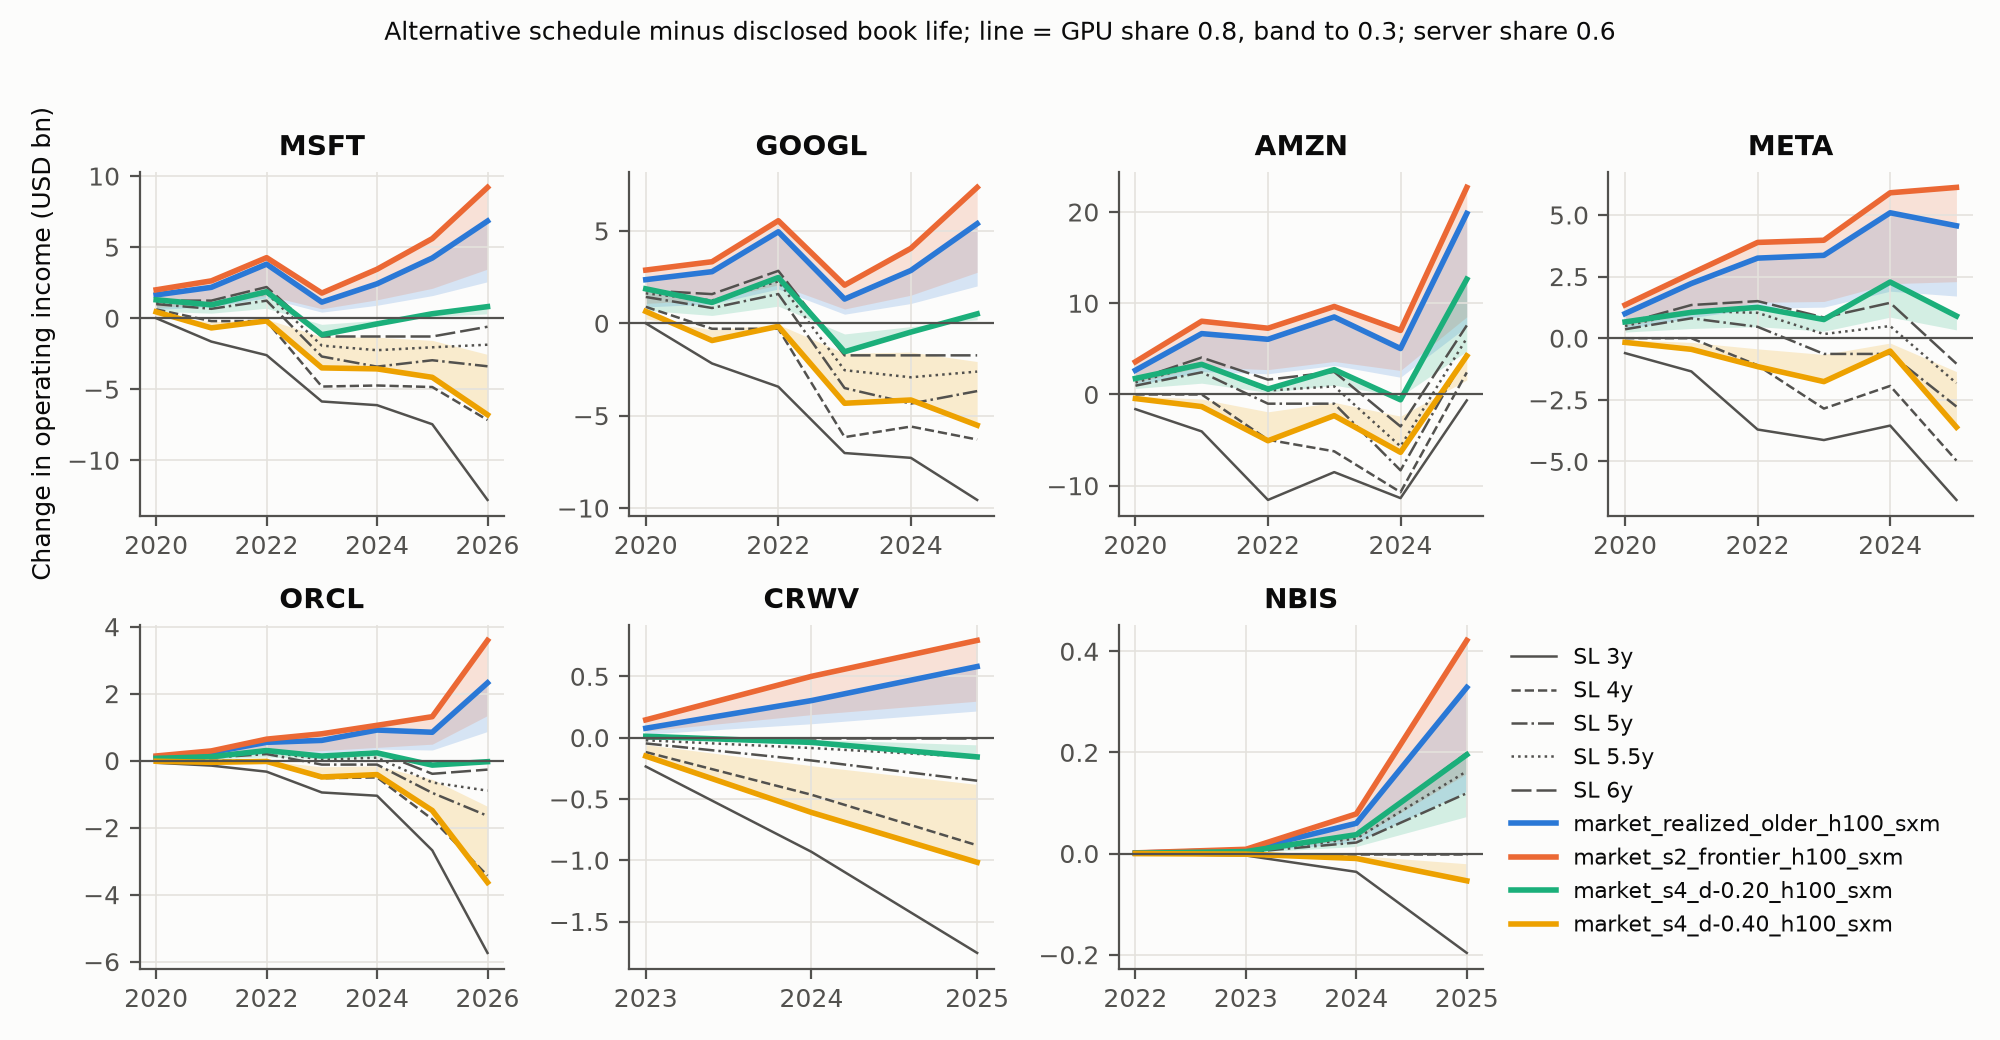
\includegraphics[width=0.85\textwidth]{p7_restatement.png}
\caption{Change in operating income by firm and schedule across the GPU-share grid.}
\label{fig:restate}
\end{figure}

\ajcheck{The sign of the restatement depends on the rent path, not on the method. Posted rents,
read through the realized paths, imply that book lives are, if anything, conservative. Only an
assumption of steep age-driven decline, which the rent data do not establish, produces the large
earnings overstatements discussed in the public debate.} The restatement inherits the limits of
the asset base: cash capital expenditure excludes finance-lease additions, which are material for
Amazon and Microsoft, and the server and GPU shares are assumptions shown as a grid.
